\documentclass[12pt, letterpaper]{article}

\usepackage{graphicx}
\usepackage{amsmath}

\title{Experiment 2 Prelab}
\author{Jay Shen}
\date{October 2024}

\begin{document}

\maketitle

\begin{figure}[h]
    \centering
    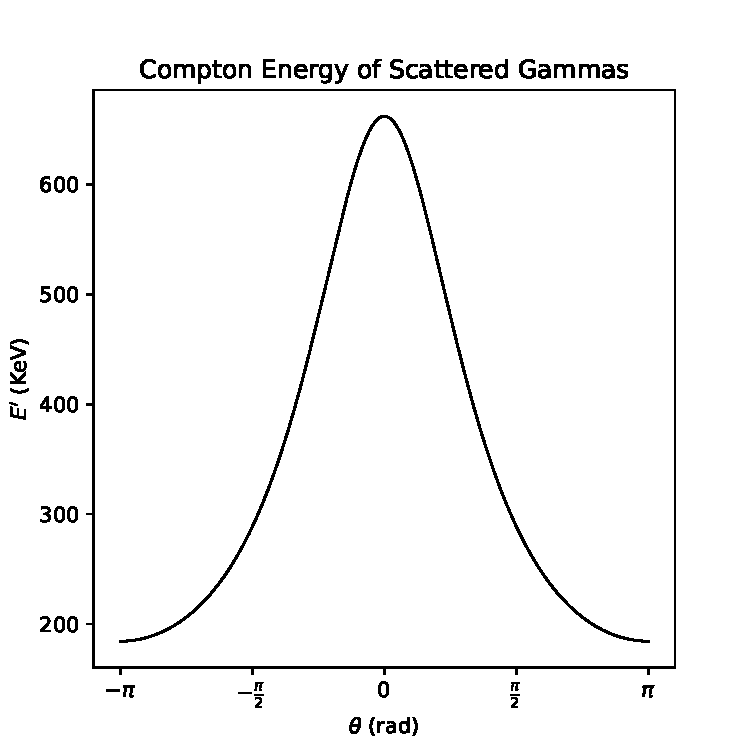
\includegraphics[width=0.5\linewidth]{experiment2/figures/compton_energy.pdf}
    \caption{Compton energy of scattered gammas versus scattering angle}
    \label{fig:compton}
\end{figure}

\begin{itemize}
    \item {
        In the plot, the scattered energy is greatest at angle $\theta=0$ and lowest at angles $\theta=\pm \pi$. 
    }
    \item {
        Now, since $E'$ is dependent on $\cos \theta$, it has $2\pi$-translational symmetry. This makes sense, as we are dealing with radial scattering. So $E'$, in general, is maximized at $\theta=2\pi n$ and minimized at $\theta=\pi (2m + 1)$ for $n, m\in \mathbb{Z}$. 
    }
    \item {
        No, the scattered energies never go to zero according to this model. This makes sense as energy is conserved and we would not expect the photon to transfer all its energy to the electron. 
    }
\end{itemize}


\end{document}
